\section{Постановка задачи}

\begin{frame}
\frametitle{Цели и задачи}
\begin{block}{Цель работы}
    Разработать веб-платформу Robbi
\end{block}

\bigskip
\pause

\begin{block}{Задачи}
    Разработать:
    \begin{enumerate}
        \item \label{itm:task:arch} Архитектуру платформы
        \item \textdim{Фронтэнд веб-сайта}
        \item \textdim{Бэкэнд}
        \item \label{itm:task:infra} Клиент для инфраструктуры ОК
    \end{enumerate}
\end{block}
\end{frame}

\begin{frame}
\frametitle{Задача \ref{itm:task:arch} Архитектура платформы}
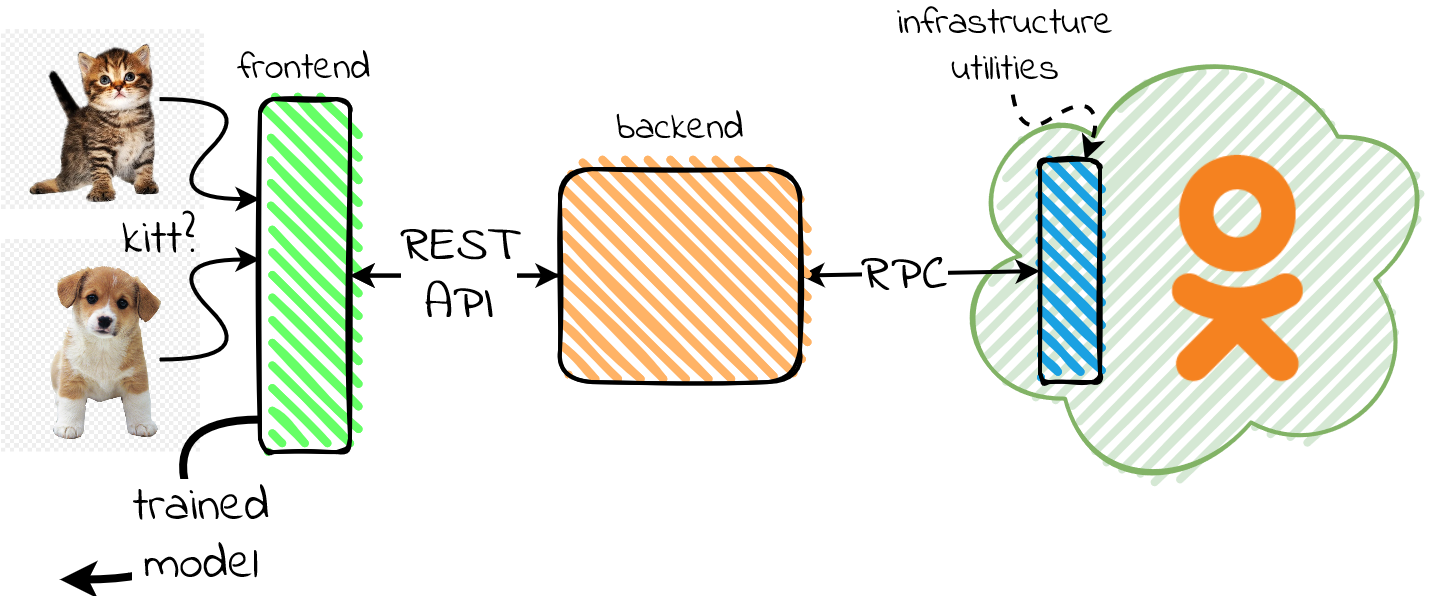
\includegraphics[width=\textwidth]{architecture.png}
\end{frame}
